\section{Designing SimpleSpeech}
Building on the capabilities developed in these prior studies, SimpleSpeech is a web-based application for recording and editing short voice messages in a discussion setting.
Our design goals were as follows: to support versatile live voice production features with a text-like interface, and to maintain a simple baseline appearance that extends into more complex features through modes and quasi-modes.
The appearance of the final SimpleSpeech user interface (UI) is shown in Fig. \ref{fig:overview_shot}.

\subsection{Text-Based Editing}
There are a wide variety of approaches to audio editing, ranging from waveform-only interfaces such as Audacity and Adobe Audition to semantic speech editors \cite{whittaker_semantic} which show only a transcript. 
For SimpleSpeech, we decided to adopt an interaction paradigm similar to the latter, allowing the user to edit a textual representation which was time-aligned with the audio.
This choice was made for two reasons: (1) in general, users are much more familiar with text than with waveform editing; and (2) representing the audio as text would greatly simplify speech editing on the word level, in contrast to the greater complexity of millisecond-level waveform operations. 

Accordingly, the UI for SimpleSpeech devotes the majority of the editing panel to the transcription. 
Users interact with the text by selecting, editing, and deleting \textit{tokens}, which are colored blue for words and green for pauses and unrecognized sounds. 
In addition to deleting tokens using the Backspace key, green pause tokens can be inserted or extended using the space bar.
Deleting and inserting tokens results in the appropriate modifications automatically applied to the working audio file.

\begin{figure}
	\centering
	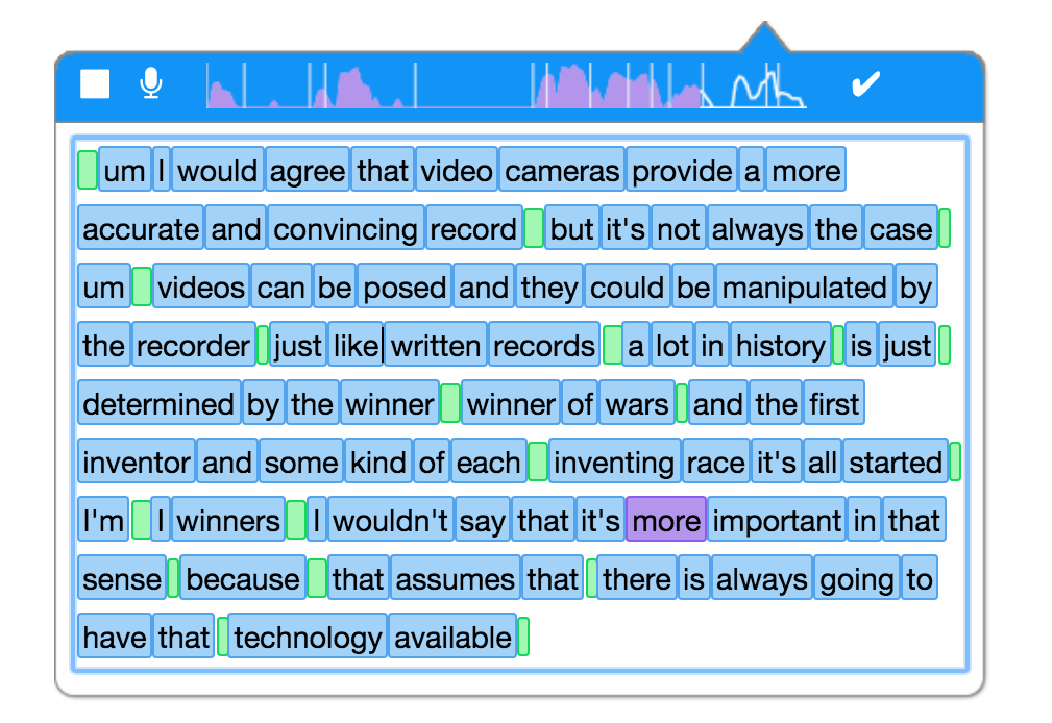
\includegraphics[width=\columnwidth,keepaspectratio]{figures/playback}
	\caption{The waveform visual at the top of the SimpleSpeech editor does not support direct millisecond-level editing; instead, it serves as a visual cue connecting the transcript to the working recording. For instance, the waveform is highlighted during playback in tandem with the current word that is being played.}~\label{fig:playback}
\end{figure}

\subsection{Reinforcing the Connection Between Audio and Text}
We chose to include a waveform visualization as part of the UI in order to remind the user that he or she is ultimately manipulating audio, not text. The waveform incorporates several subtle indications of the mapping between its contents and the transcription, including highlighting the audio corresponding to the current selection of tokens and animating deletions and insertions.
We found the presence of a waveform to be a helpful visual indicator of the purpose of SimpleSpeech, although it was not functionally useful \textit{per se}.
Without the waveform, users' inclination was to disregard the original speech and use the system as a dictation tool.

Another strategy to reinforce the parallelism between the source audio and the transcription is to highlight the words in the transcript as they are spoken during playback, as shown in Fig. \ref{fig:playback}.
The waveform renders the portion of audio that has already been played in a purple color, which is also used to render the token currently being played back.

\subsection{Editing Audio vs. Fixing Transcription Errors}
Our use of text as a proxy for editing audio rendered it necessary to clearly delineate the capabilities of SimpleSpeech in comparison to a word processor.
For instance, direct text input is disallowed in the transcript area to avoid inserting words not present in the original recording.
(The inability to move the caret within the tokens visually confirms that the transcript cannot be edited without correspondence to the audio.)
However, we found the capability to edit text of individual words in the transcript to be desirable, especially in the case of ASR errors.
As shown in Fig. \ref{fig:transcription}, the transcription editing functionality is available in a separate mode, accessed by pressing the Return key.
The pop-up box insulates the editing within single words to avoid undermining the cohesiveness of the tokens. 
(If the user starts typing while one or more tokens were selected, this automatically activates the transcription editing mode as well; some pilot users found this more intuitive than using the Return key.)

\begin{figure}
	\centering
	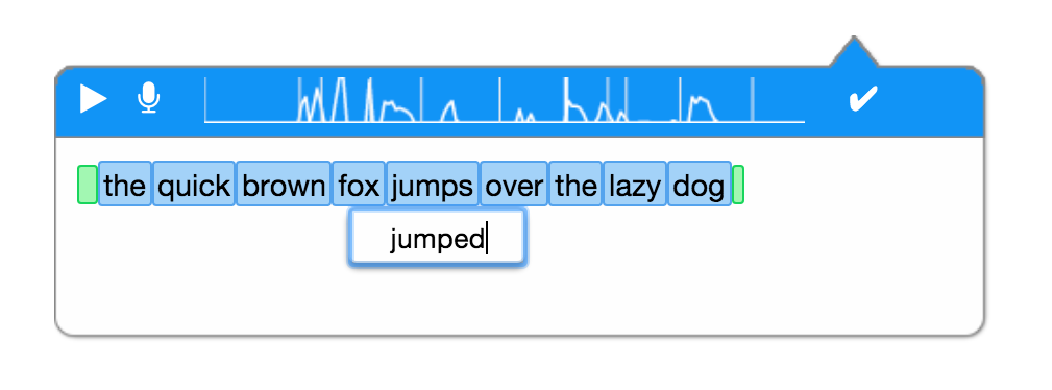
\includegraphics[width=\columnwidth,keepaspectratio]{figures/transcription_edit}
	\caption{To keep the user interface from becoming cluttered with secondary functionality, the transcription editing feature was implemented as a modal interaction. The pop-up box shown above ``opens'' the selected tokens for text editing in a separate control element, thus notifying the user that he or she is no longer directly editing the audio.}~\label{fig:transcription}
\end{figure}

\subsection{Pilot Study and Design Improvements}
We followed an iterative procedure to progressively improve the design and interactions of SimpleSpeech.
After building an initial prototype of the application, an informal pilot test was conducted with 5 participants (4 female, 1 male). 
Each user was given a brief introduction to the software and shown how to use the basic features, then given the scenario of creating an audio response to a written claim on an online forum. 
(The prompts used in the tests were adapted from the GRE Pool of Issue Topics.)
After using the software, users were interviewed to obtain feedback on the prototype, yielding the following modifications:

\emph{Playback shortcut}.
During pilot testing the need arose for a fast way to play back and pause the audio; however, the conventional keyboard shortcut for playback, the spacebar, was already in use for the pause insertion feature.
We resolved this problem by using Shift+space for playing and pausing.
In effect, the playback functionality was encapsulated as a \emph{quasi-mode}, a set of distinct features that are accessed while performing a constant action (in this case, pressing the Shift key) \cite{raskin}. 
The modal design helps prevent beginning users from being overwhelmed with possible actions while allowing more advanced users rapid access to the higher-level features.

\emph{Pause manipulation}.
Another important finding in the pilot study was the importance of being able to introduce and adjust pauses between words, not just to remove them. 
These gaps in the audio help make natural-sounding cuts between audio clips as well as to punctuate claims (e.g., the end of a sentence). 
The original system only allowed the user to delete pauses, so we added a spacebar action to insert a zero audio signal or fragment of silence from the original audio resource into the rendered message. 

\emph{Tokenization}. 
The way we had tokenized the transcript originally, the user was able to ``enter'' the tokens with the caret and change their contents.
However, this inline transcript editing behavior confused the pilot study participants, who tried to insert new unrecorded content by typing. 
We endeavored to clarify these delineations in the next iteration by disabling direct alphanumeric input to the transcript view, and shifting the transcription editing functionality into a modal interaction.

\subsection{Implementation}
Our text-based approach requires a reliable transcription as well as time intervals corresponding to each word; both of these requirements are fulfilled by the IBM Watson Developer Cloud speech-to-text transcription service, which is reported to have a word error rate of 10.4\% \cite{soltau:2014}.
For the sake of the cross-platform compatibility, the application was implemented as a web app written in JavaScript, HTML, and CSS.
Editing is accomplished by maintaining a data model consisting of one or more user-created audio resources as well as a list of timestamps, each of which links a token in the text area to a time interval within an audio resource. 
When the user plays back the message, the data model ``renders'' a complete audio recording by stitching together the audio from each timestamp. 
